A fit to the \mll distribution is performed in search of the characteristic edge signature described in section~\ref{sec:somesignalsection}. Different functions are used to model the contributions of the potential signal, flavour-symmetric backgrounds, and backgrounds containing a Z boson. To fully exploit the available information, an unbinned maximum-likelihood fit is performed simultaneously to the \EE, \MM, and \EM event samples for both the signal and forward dilepton selection in the signal region.

\section{Signal and background models}
\subsection{Signal model}
While the shape of the signal depends on the details of the signal model, deviations from a simple triangular shape are small compared to the detector resolution. The signal is therefore modelled by such a triangle, convolved with a Gaussian distribution. The width of the Gaussian $\sigma_{\ell\ell}$ depends on the detector resolution and is chosen to be $\unit{1}{\giga\electronvolt}$ for \MM and $\unit{2}{\giga\electronvolt}$ for \EE events based on studies on simulation\fixme{find out how Daniel did this and repeat study}. The model can be parametrized as
\begin{equation*}
 {\mathcal{P}}_{S}(m_{\ell\ell}) = \frac{1}{\sqrt{2\pi\sigma_{\ell\ell}}} \int_{0}^{m_{\ell\ell}^{edge}} y \cdot \textrm{exp}\left( -\frac{(m_{\ell\ell}-y)^2}{2\sigma_{\ell\ell}^{2}}\right) dy,
\end{equation*}
with the endpoint of the triangle $m_{\ell\ell}^{edge}$ as the only free parameter.

\subsection{Model for Z backgrounds}
The background for containing a Z boson contains of two components: one model for the Z boson peak and one for the contribution of the Drell--Yan continuum. The latter one is a simple falling exponential. The peak model consists of a Breit-Wigner function with mean and widths fixed to the DPG values for the Z boson, convolved with a double-sided crystal ball function~\cite{Crystal}. The first component models the physical peak while the latter accounts for the detector resolution and radiative corrections to the Z lineshape. The double-sided crystal ball itself consists of a Gaussian core and exponential falloffs to both sides of the peak, parametrized as
\begin{eqnarray*}
\mathcal{P}_{DSCB}(m_{\ell\ell}) = \begin{cases} A_{1} (B_{1}-\frac{m_{ll}-\mu_{CB}}{\sigma_{CB}})^{-n_{1}} &\mbox{if } \frac{m_{ll}-\mu_{CB}}{\sigma_{CB}}<-\alpha_{1} \\
\textrm{exp}\left(-\frac{(m_{ll}-\mu_{CB})^2}{2\sigma_{CB}^2}\right) &\mbox{if } -\alpha_{1}<\frac{m_{ll}-\mu_{CB}}{\sigma_{CB}}<\alpha_{2} \\
A_{2} (B_{2}+\frac{m_{ll}-\mu_{CB}}{\sigma_{CB}})^{-n_{2}} &\mbox{if } \frac{m_{ll}-\mu_{CB}}{\sigma_{CB}}>\alpha_{2} \\
\end{cases}
\end{eqnarray*}
where $\sigma_{CB}$ and $\mu_{CB}$ are the parameters of the central Gaussian and the $n_i$ and $\alpha_i$ govern the transition to and the shape of the exponential falloff. The $A_i$ and $B_i$ are substitutions for
\begin{eqnarray*}
A_{i} = \left(\frac{n_{i}}{|\alpha_{i}|}\right)^{n_{i}} \cdot \textrm{exp}\left(-\frac{|\alpha_{i}|^2}{2}\right) \quad \textrm{and}\quad B_{i} = \frac{n_{i}}{|\alpha_{i}|}-|\alpha_{i}| .
\end{eqnarray*}
Taking into account also the exponential function described the Drell--Yan continuum, the full description is therefore 
\begin{eqnarray*}
\mathcal{P}_{DY} (m_{\ell\ell}) = f_{exp}\mathcal{P}_{exp}(m_{\ell\ell})+(1-f_{exp})\int \mathcal{P}_{DSCB}(m_{\ell\ell})\mathcal{P}_{BW}(m_{\ell\ell}-m') dm',
\end{eqnarray*}
where $f_{exp}$ is the fraction that the exponential component contributes to the full PDF. 

This model is fitted to the data in the Drell--Yan control region separately for \EE and \MM events after flavour-symmetric backgrounds are subtracted using OF events. Afterwards, all parameters of the model are fixed and only the normalization is left floating in the fit in the signal region. The resulting fits are shown in Figure~\ref{fig:dyFits} and are a good description of the distribution in all cases. 

\begin{figure}[htbp]
\centering
\begin{minipage}[t]{0.49\textwidth}
  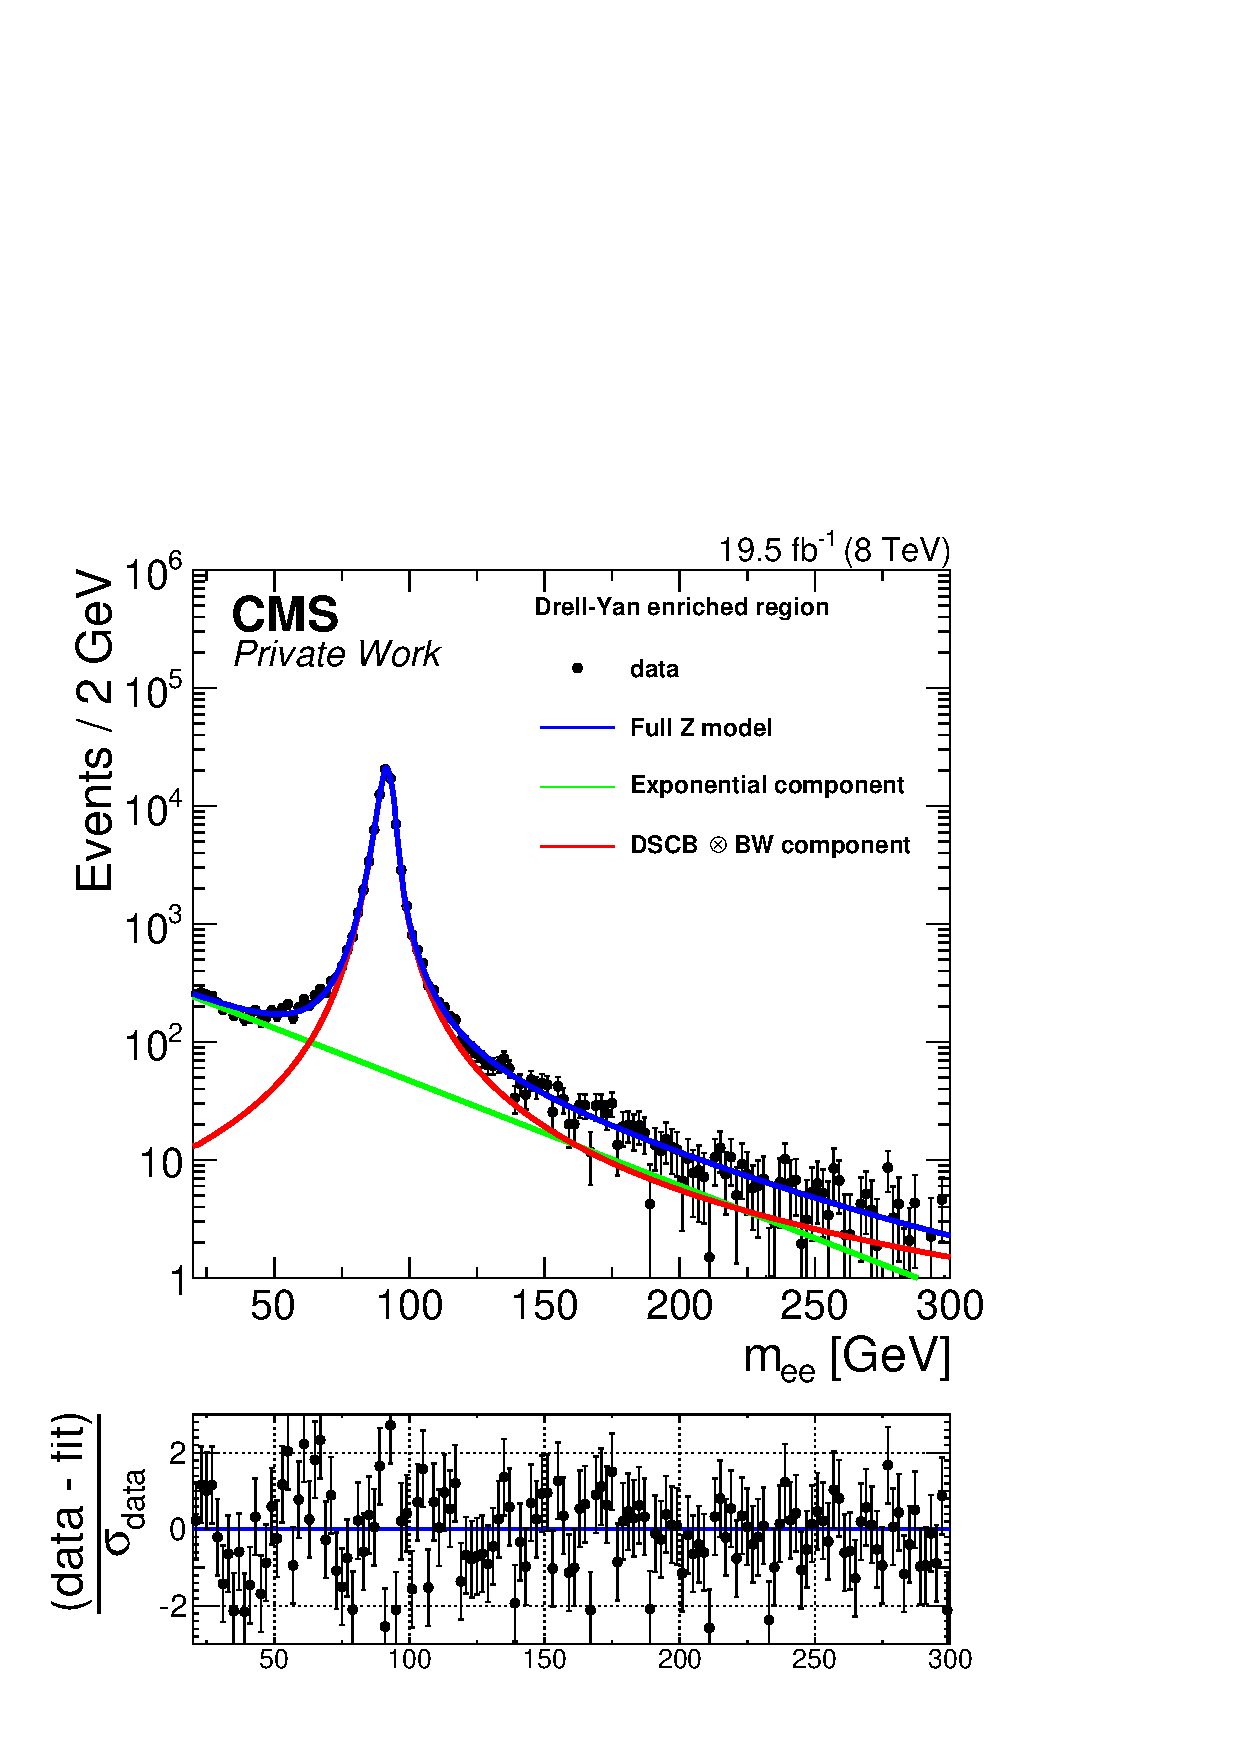
\includegraphics[width=\textwidth]{plots/results/fit/expoFitEE_Log_Central.pdf}
\end{minipage}
\begin{minipage}[t]{0.49\textwidth}
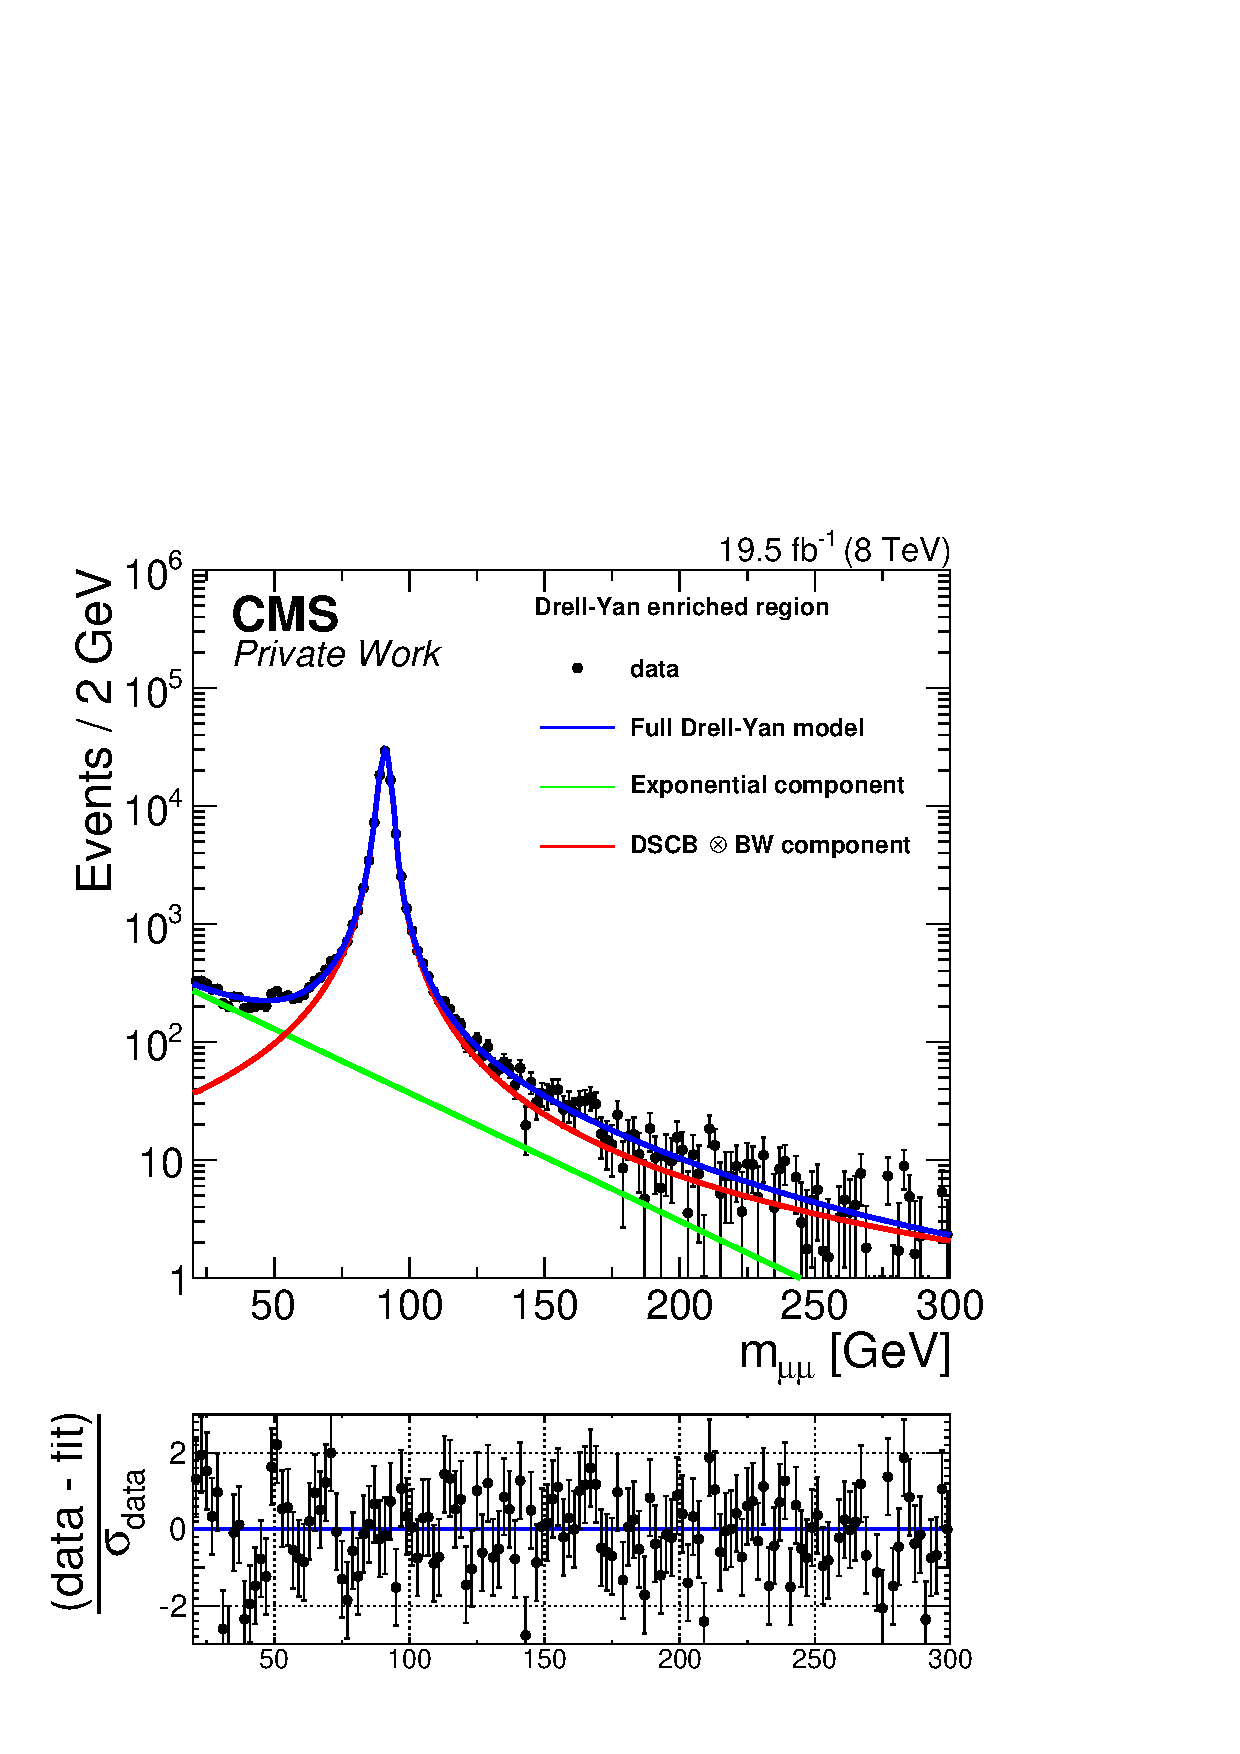
\includegraphics[width=\textwidth]{plots/results/fit/expoFitMM_Log_Central.pdf}
\end{minipage}
\begin{minipage}[t]{0.49\textwidth}
  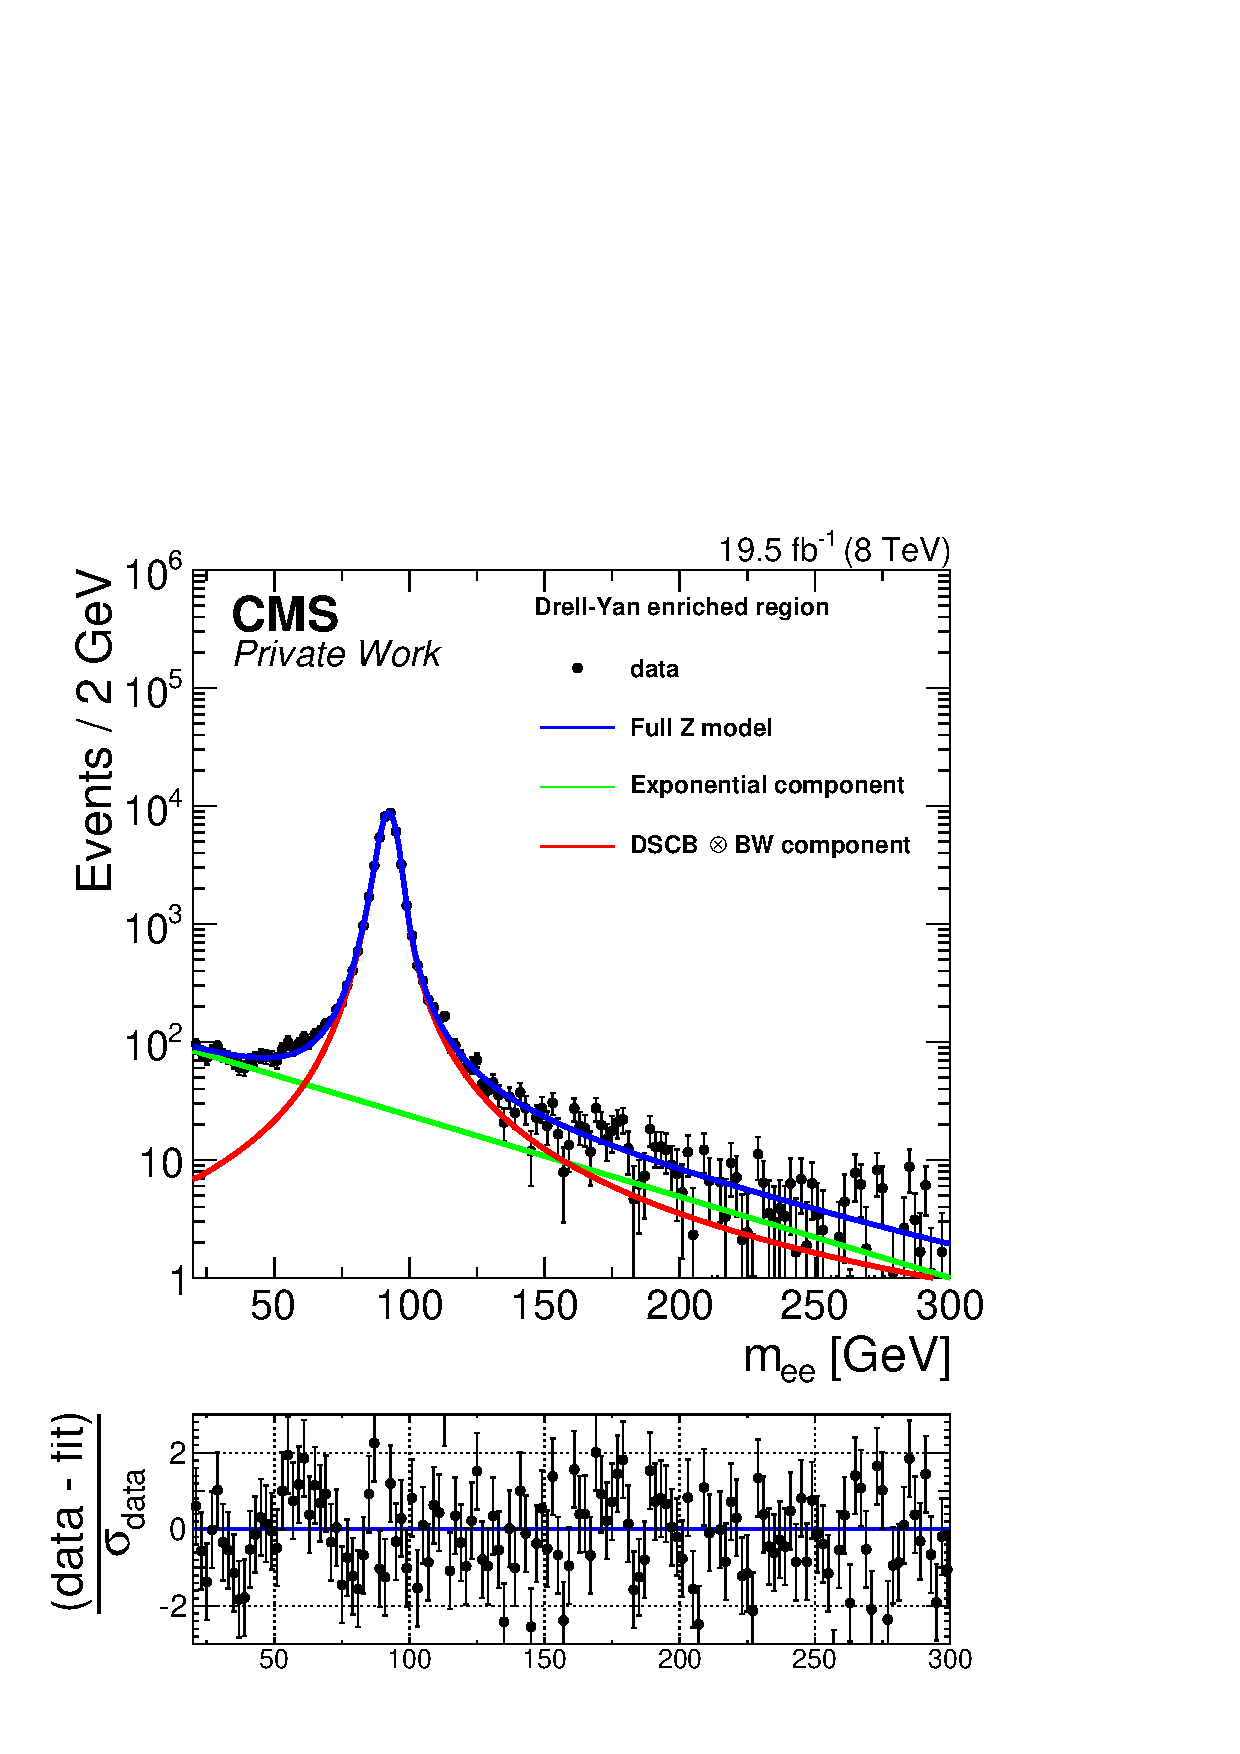
\includegraphics[width=\textwidth]{plots/results/fit/expoFitEE_Log_Forward.pdf}
\end{minipage}
\begin{minipage}[t]{0.49\textwidth}
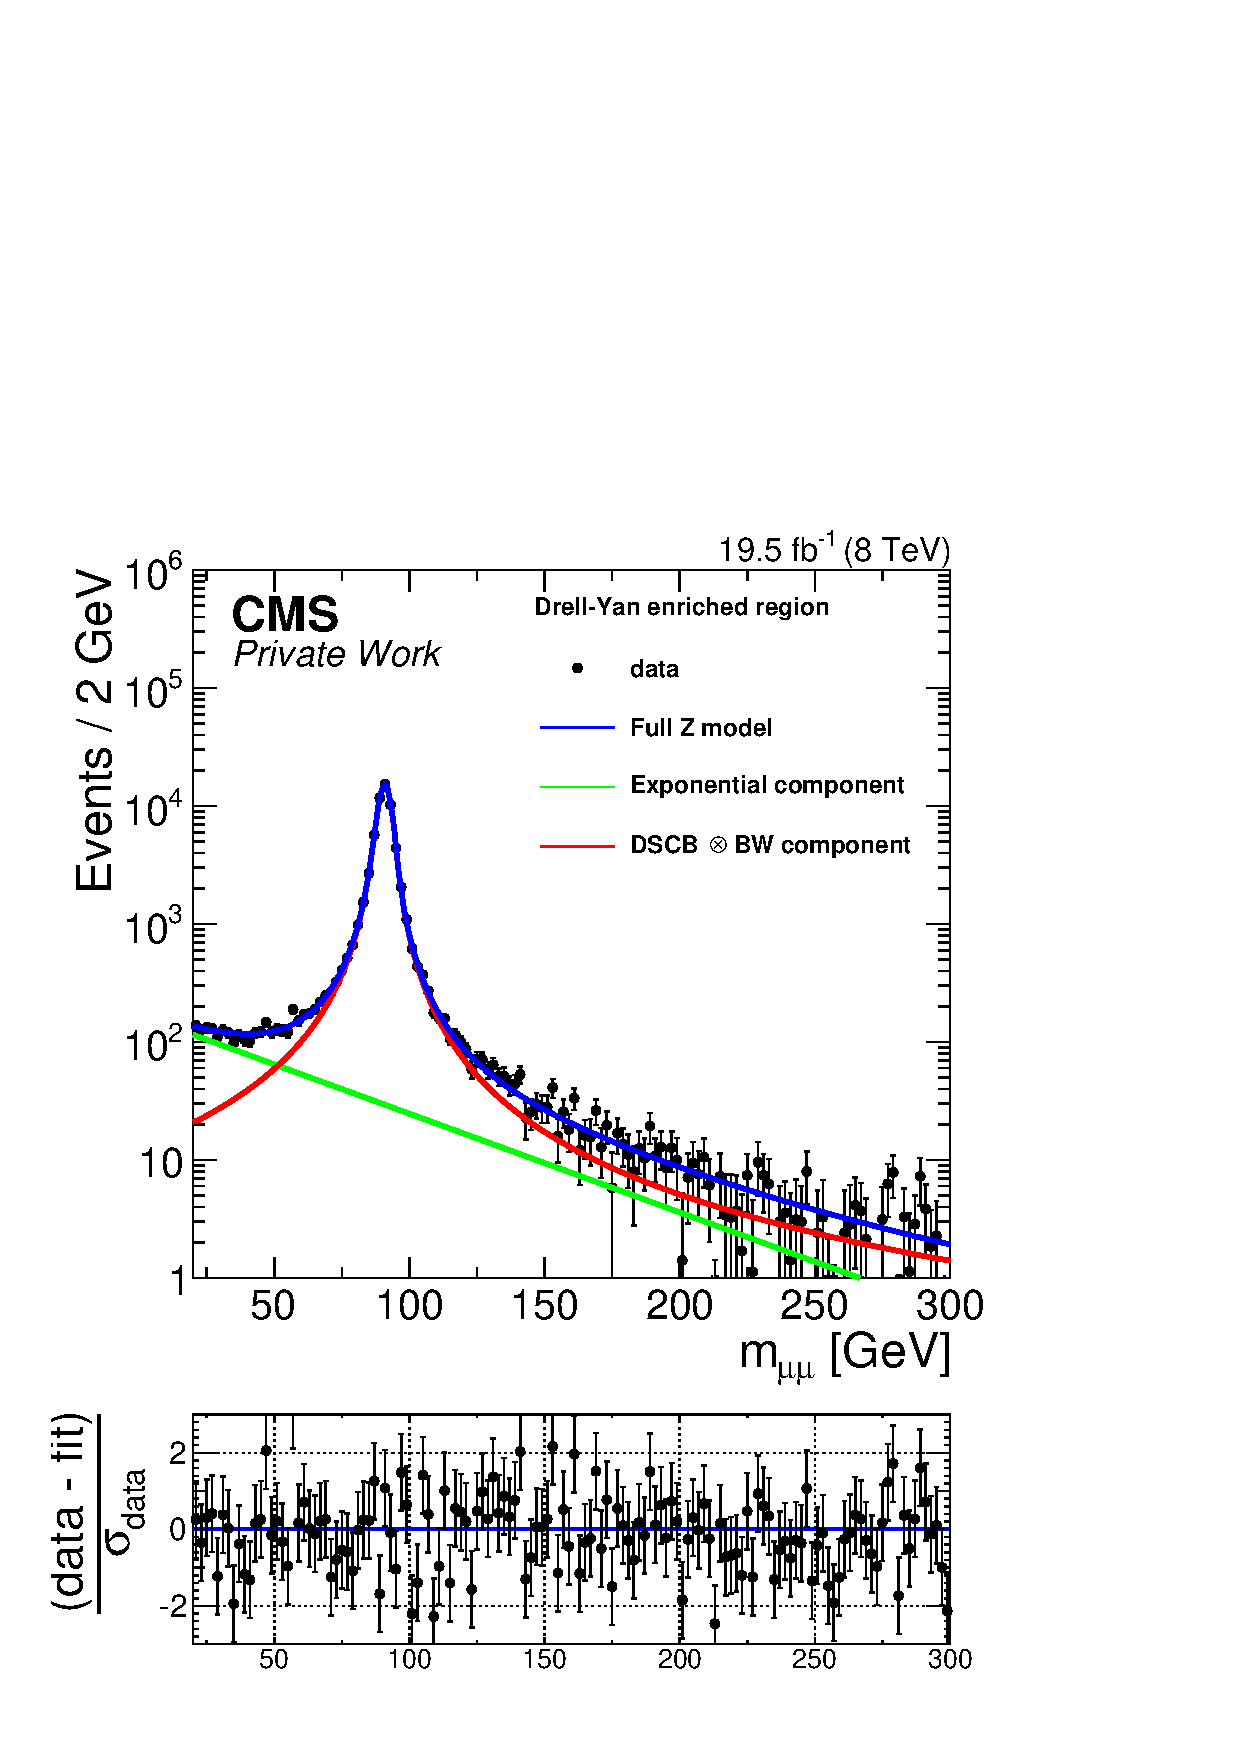
\includegraphics[width=\textwidth]{plots/results/fit/expoFitMM_Log_Forward.pdf}
\end{minipage}
\caption{Fit to the \mll distribution in the Drell--Yan control region separately for \EE (left) and \MM (right) events in the central (top) and forward (bottom) dilepton selection. The data is shown as black points while the resulting fit is shown in blue. The red and green lines show the contributions of the continuum model and the peak model to the combined fit.}
\label{fig:dyFits}
\end{figure}


\subsection{Model for flavour-symmetric backgrounds}

\subsubsection{Default parametrization}
Flavour-symmetric models are described with a model consisting of three parts. The rising flank of the distribution is modelled with a power law, the peak region with a fourth order polynomial and the falling flank with an exponential falloff. 

\begin{eqnarray*}
{\mathcal{P}}_{FSE}(m_{\ell\ell}) = \begin{cases} {\mathcal{P}}_{FSE,1}(m_{\ell\ell}) = c_{1} \cdot m_{\ell\ell}^{\alpha} &\mbox{if } 20\GeV < m_{\ell\ell} < m_{\ell\ell}^{(1)} \\
{\mathcal{P}}_{FSE,2}(m_{\ell\ell}) = \sum_{i=0}^{3} c_{2,i} \cdot m_{\ell\ell}^{i} & \mbox{if } m_{\ell\ell}^{(1)}<m_{\ell\ell}<m_{\ell\ell}^{(2)} \\
{\mathcal{P}}_{FSE,3}(m_{\ell\ell}) = c_{3}\cdot e^{-\beta m_{\ell\ell}} & \mbox{if } m_{\ell\ell}^{(2)}<m_{\ell\ell}<300\GeV \\
\end{cases} 
\end{eqnarray*}
where $m_{\ell\ell}^{(1)}$ and $m_{\ell\ell}^{(2)}$ are the transition points between the different parts of the model. The model is required to be normalized and also to be continuously differentiable in $m_{\ell\ell}^{(1)}$ and $m_{\ell\ell}^{(2)}$, reducing the number of free parameters. 


A variety of alternative models for the flavour-symmetric has been explored to validate the results obtained with the model described above. 

\paragraph{Parametrization from 2011 analysis}\mbox{} \\
This parametrization was used in a previous version of the analysis~\cite{edge2011}: 
\begin{equation*}
 \mathcal{P_{FSE}}(m_{\ell\ell}) = c_{1} m_{\ell\ell}^{\alpha} e^{-\beta m_{\ell\ell}}
\end{equation*}
It was found to not describe the distrubtion of flavour-symmetric backgrounds after lepton \pt cuts had been raised with respect to the analysis of the 2011 dataset, but is still a useful tool for fit performance studies, as the low number of parameters reduce the runtime of the fit, allowing for tests using a large number of toy datasets.
\paragraph{Sum of three Gaussians}\mbox{} \\
In this case the sum of three Gaussians is chosen as an analytical parametrization of the flavour-symmetric backgrounds. The free parameters of the shape are the means and widths of the Gaussians.
\begin{equation*}
\mathcal{P_{FSE}}(m_{\ell\ell}) = Gauss(mean_1,\sigma_1) + Gauss(mean_2,\sigma_2) + Gauss(mean_3,\sigma_3)\\
\end{equation*}
The shape is found to well describe the flavour-symmetric background and to be in good agreement with the default parametrization.
\paragraph{Binned Subtraction}\mbox{} \\


\label{shapesubtraction:binnedsubtraction}

As an alternative to analytical functions, the binned dilepton-mass distribution in the OF channel is directly used as  template of the distribution of flavour-symmetric backgrounds in the same-flavour channels. This results in a bin-by-bin subtraction of the flavour-symmetric background estimation from same-flavour yields taking into account the \Rsfof correction factor, similar to the counting experiment.

This approach has the advantage of not needing any prior knowledge on the shape of the flavour-symmetric background. It is however more susceptible to statistical fluctuations, as they are not smoothed out. In order to minimize the impact of these fluctuations, a bin width of 20\GeV is chosen. This method is not suited to provide quantitative results because the statistical uncertainties on shape are not considered in the fit after it has been fixed on the OF data.

\paragraph{Smoothed Subtraction}\mbox{} \\
Similarly to the binned subtraction, the opposite flavour data distribution is directly used to predict the background in the same flavour distribution. The shape is constructed by adding one Gaussian distribution at the corresponding value of \mll for each event in the dataset using a one-dimensional kernel pdf (\emph{RooKeysPdf} class in RooFit). In this approach, the probability density function for a sample of a random variable of size $n$ is estimated by a kernel density

\begin{equation}
\hat{f}_h(x) = \frac{1}{nh}\sum\limits_{i=1}^n K(\frac{x-x_i}{h}).
\end{equation}
Here $K$ is the so called kernel, for which a normal distribution is chosen, and $h$ is a smoothing parameter\cite{kernelDensity}. The width of the gaussians is adapted depending on the density of entries at a given point. For both borders, the low-$m_{\ell\ell}$ and the high-$m_{\ell\ell}$ border, parts the gaussians extending beyond the considered range of $m_{ll}$ are mirrored back into the considered range to get the correct integral. Again,this method is not suited to provide quantitative results because no uncertainties on the background shape can be included because it is already fixed prior to the fit.  

\section{Fit validation}

\subsection{Fit performance studies using toy MC}
\label{sec:toys}
The performance of the fit is studied using toy datasets. These are generated by fitting the background shape for flavour-symmetric backgrounds to OF im simulation. From this shape new opposite-flavour datasets are generated, fluctuating the normalization using a Poisson distribution. Electron-electron and muon-muon datasets are generated by adding the \Z peak model, normalized to the combined JZB and $E_T^{miss}$-template prediction. The \Z and flavour-symmetric yield is split into these two datasets using the \rmue value measured in data and fluctuated independently. If desired, a signal is injected in the same-flavour datasets in a similar fashion. The combined fit is performed on these datasets. As the nominal background shape is quite resource intensive, the parametrization from the 2011 analysis is used in this studies in order to generate sufficient statistics for these studies. 
\paragraph{Toy studies without signal injection}
The edge fit is performed on toys generated from the background models only. Figure~\ref{fig:toys:backgroundOnly} shows resulting distributions for the fitted number of signal events in the central region. The left plot shows just the number of fitted signal events, distributed roughly as a Gaussian around 0. On the right the number of fitted signal events divided by the fitted uncertainty is shown. The distribution exhibits two peaks, symmetrically below and above zero. This feature is caused by the fact the the edge position is a floating parameter in the fit. As the fit will choose an edge position for which the likelihood is improved the most when the signal model is included compared to the background only model, this biases the fit towards more significant signals. Figure~\ref{fig:toys:backgroundOnlyFixed} shows the results for fits to background only toys but with fixed position of the edge. As can be seen on the right, the distribution of $N_{sig}/\sigma_{N_{sig}}$ is now a unit Gaussian centred around zero, as one would expect in the absence of a signal. 
\begin{figure}[hbp]
  \centering
  \begin{minipage}[t]{0.49\textwidth}
    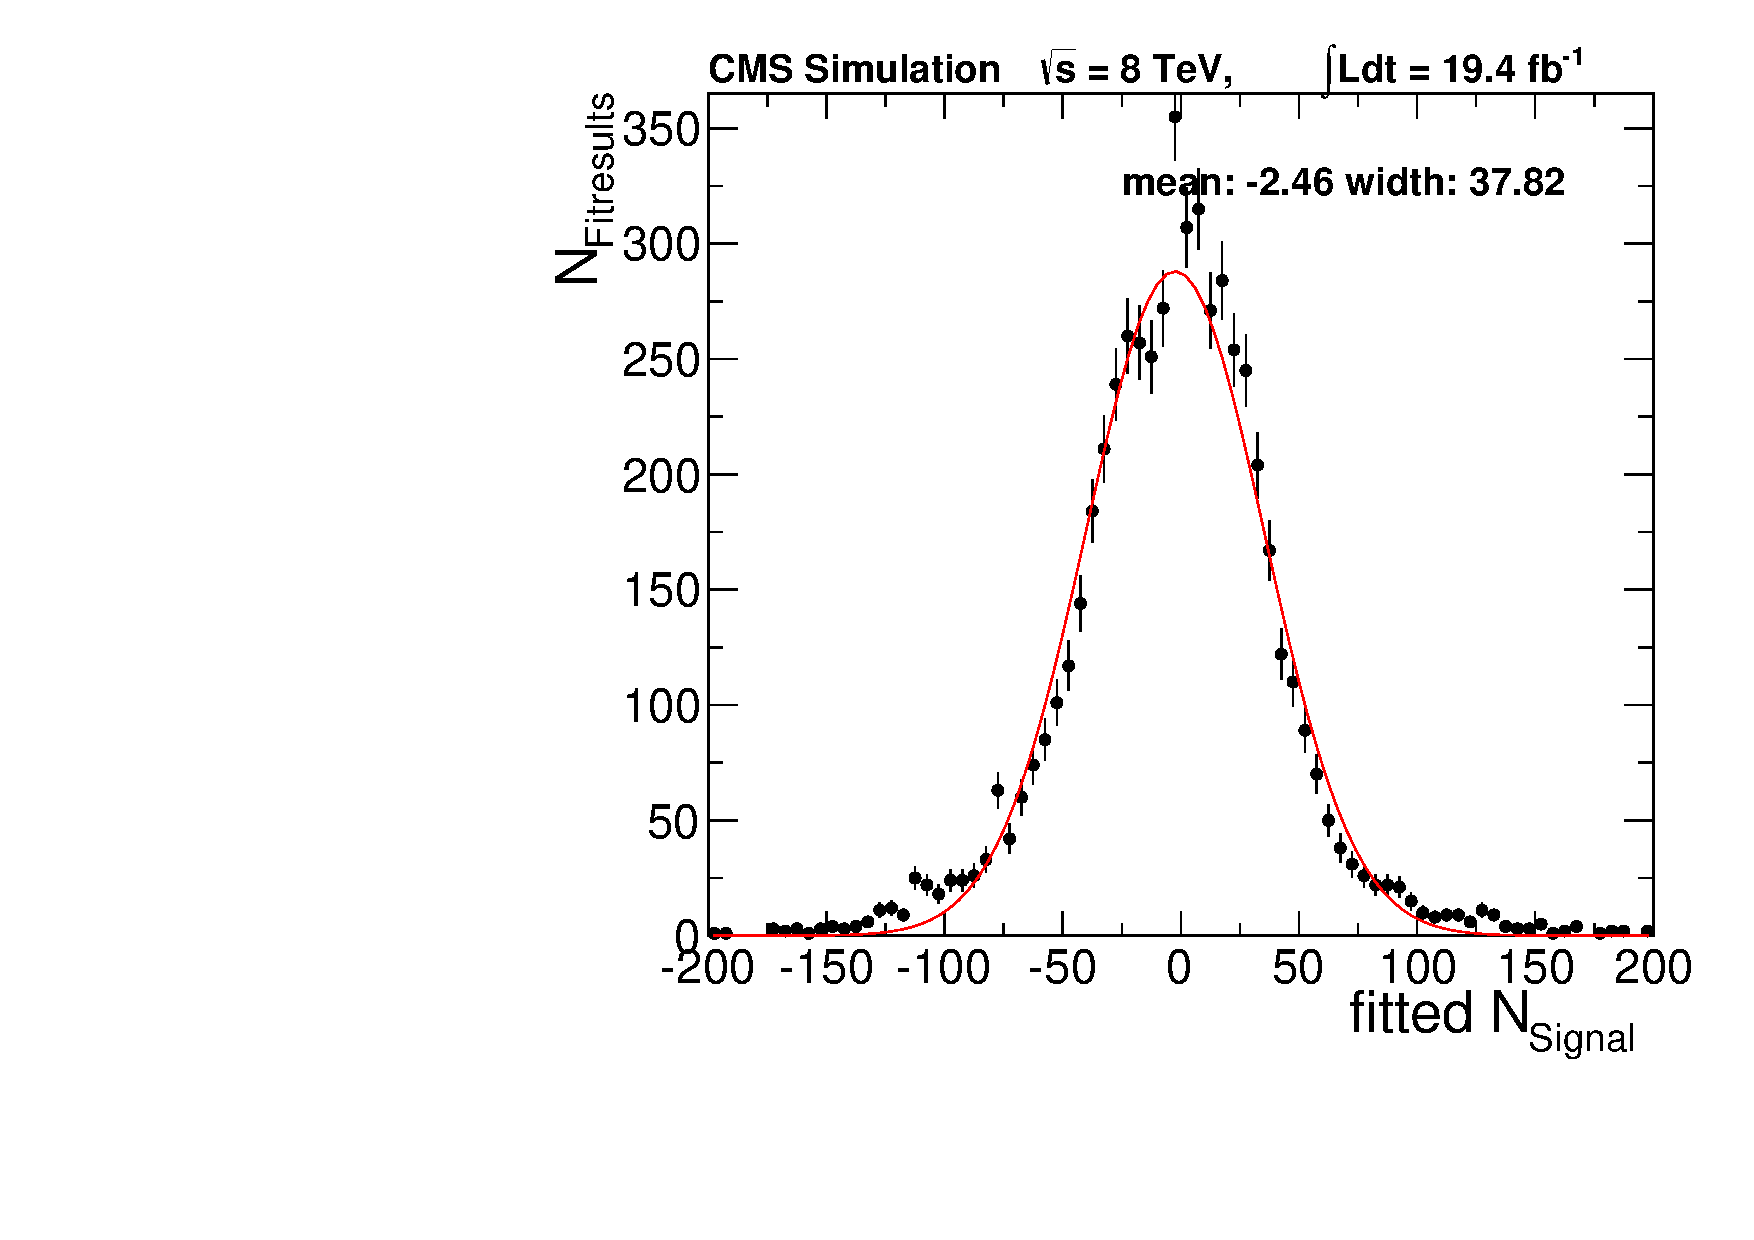
\includegraphics[width=\textwidth]{plots/results/fit/nSPure_backgroundOnly_m040.pdf}
  \end{minipage}
  \begin{minipage}[t]{0.49\textwidth}
    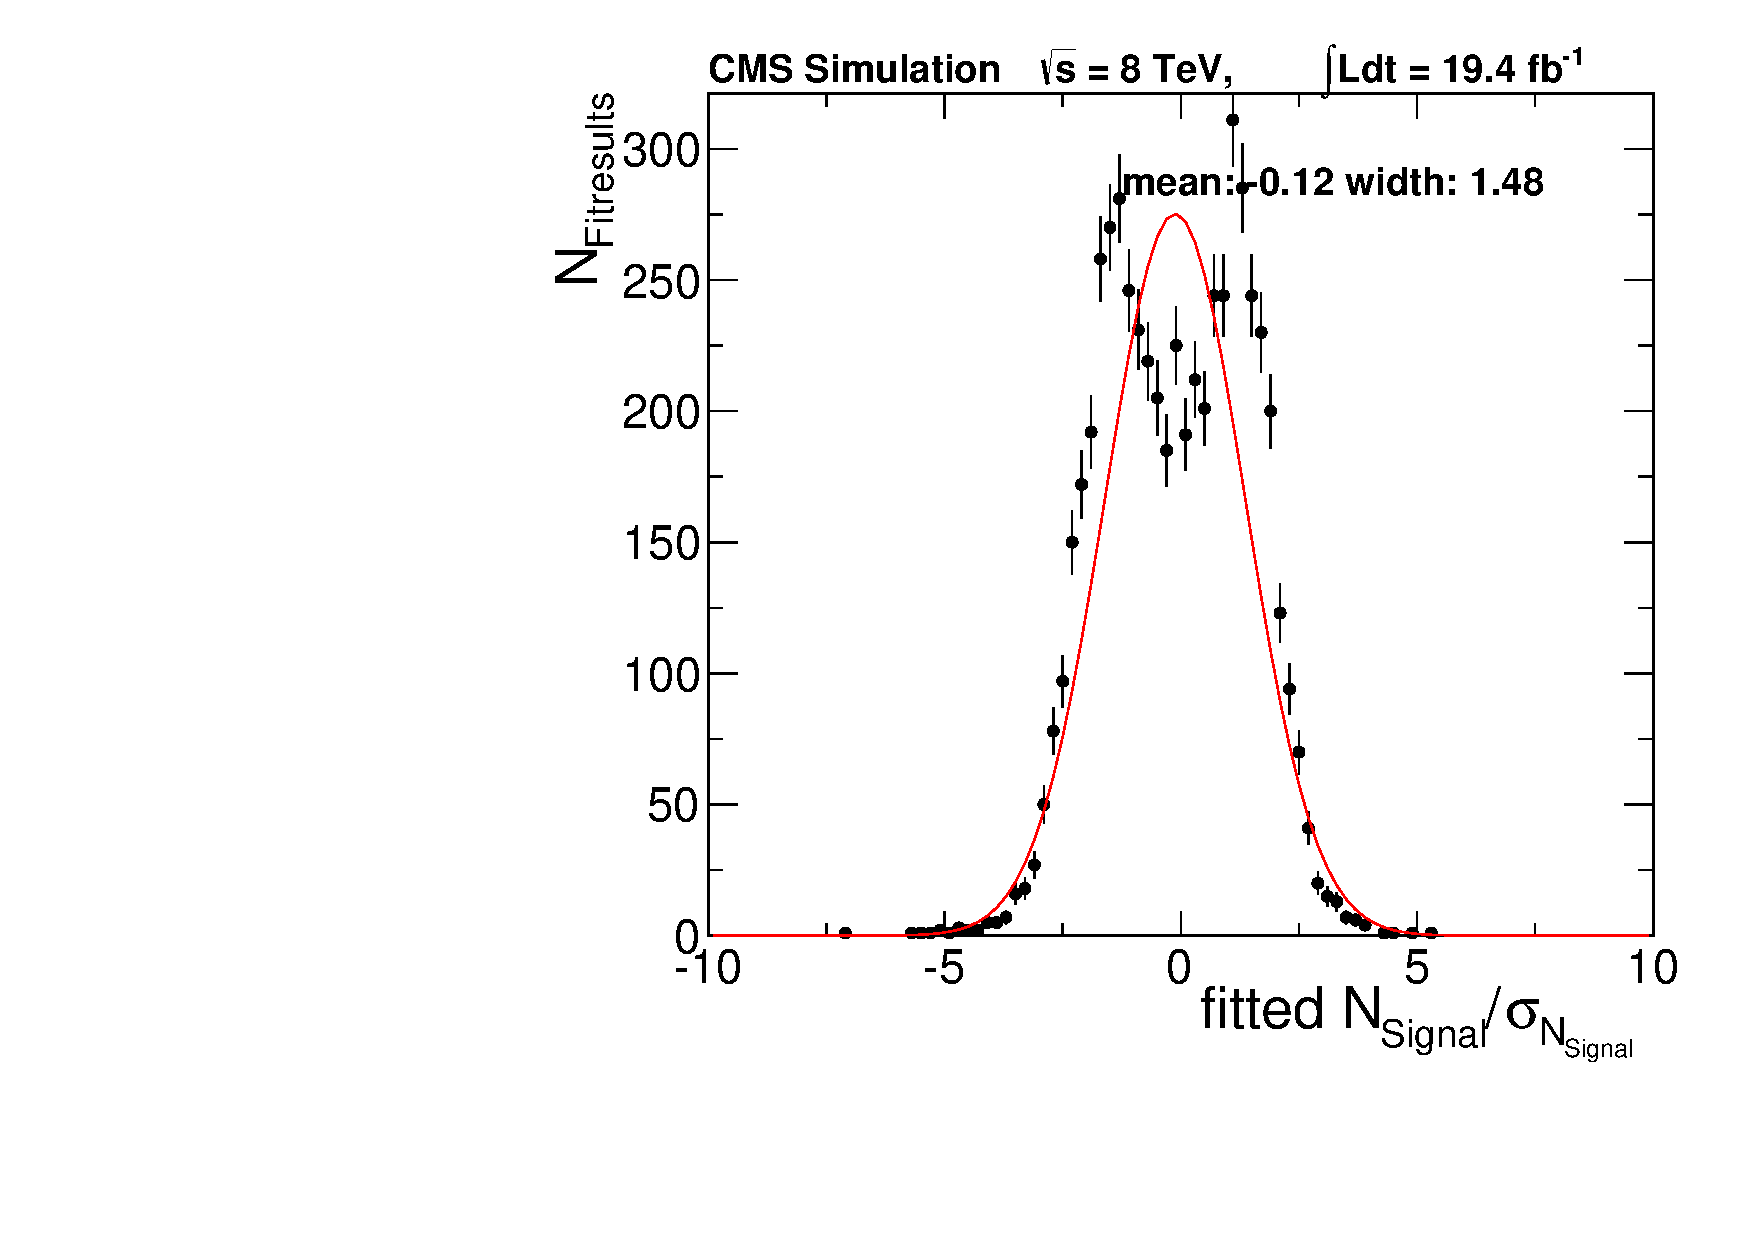
\includegraphics[width=\textwidth]{plots/results/fit/nS_backgroundOnly_m040.pdf}
  \end{minipage}

  \caption{Distribution of fit observables in toy studies for background only toys. Shown are the fitted number of signal events in the central region (left) and the fitted number of signal events divided by the fitted uncertainty in the central region (right).}
  \label{fig:toys:backgroundOnly}
\end{figure}
\begin{figure}[hbp]
  \centering
  \begin{minipage}[t]{0.49\textwidth}
    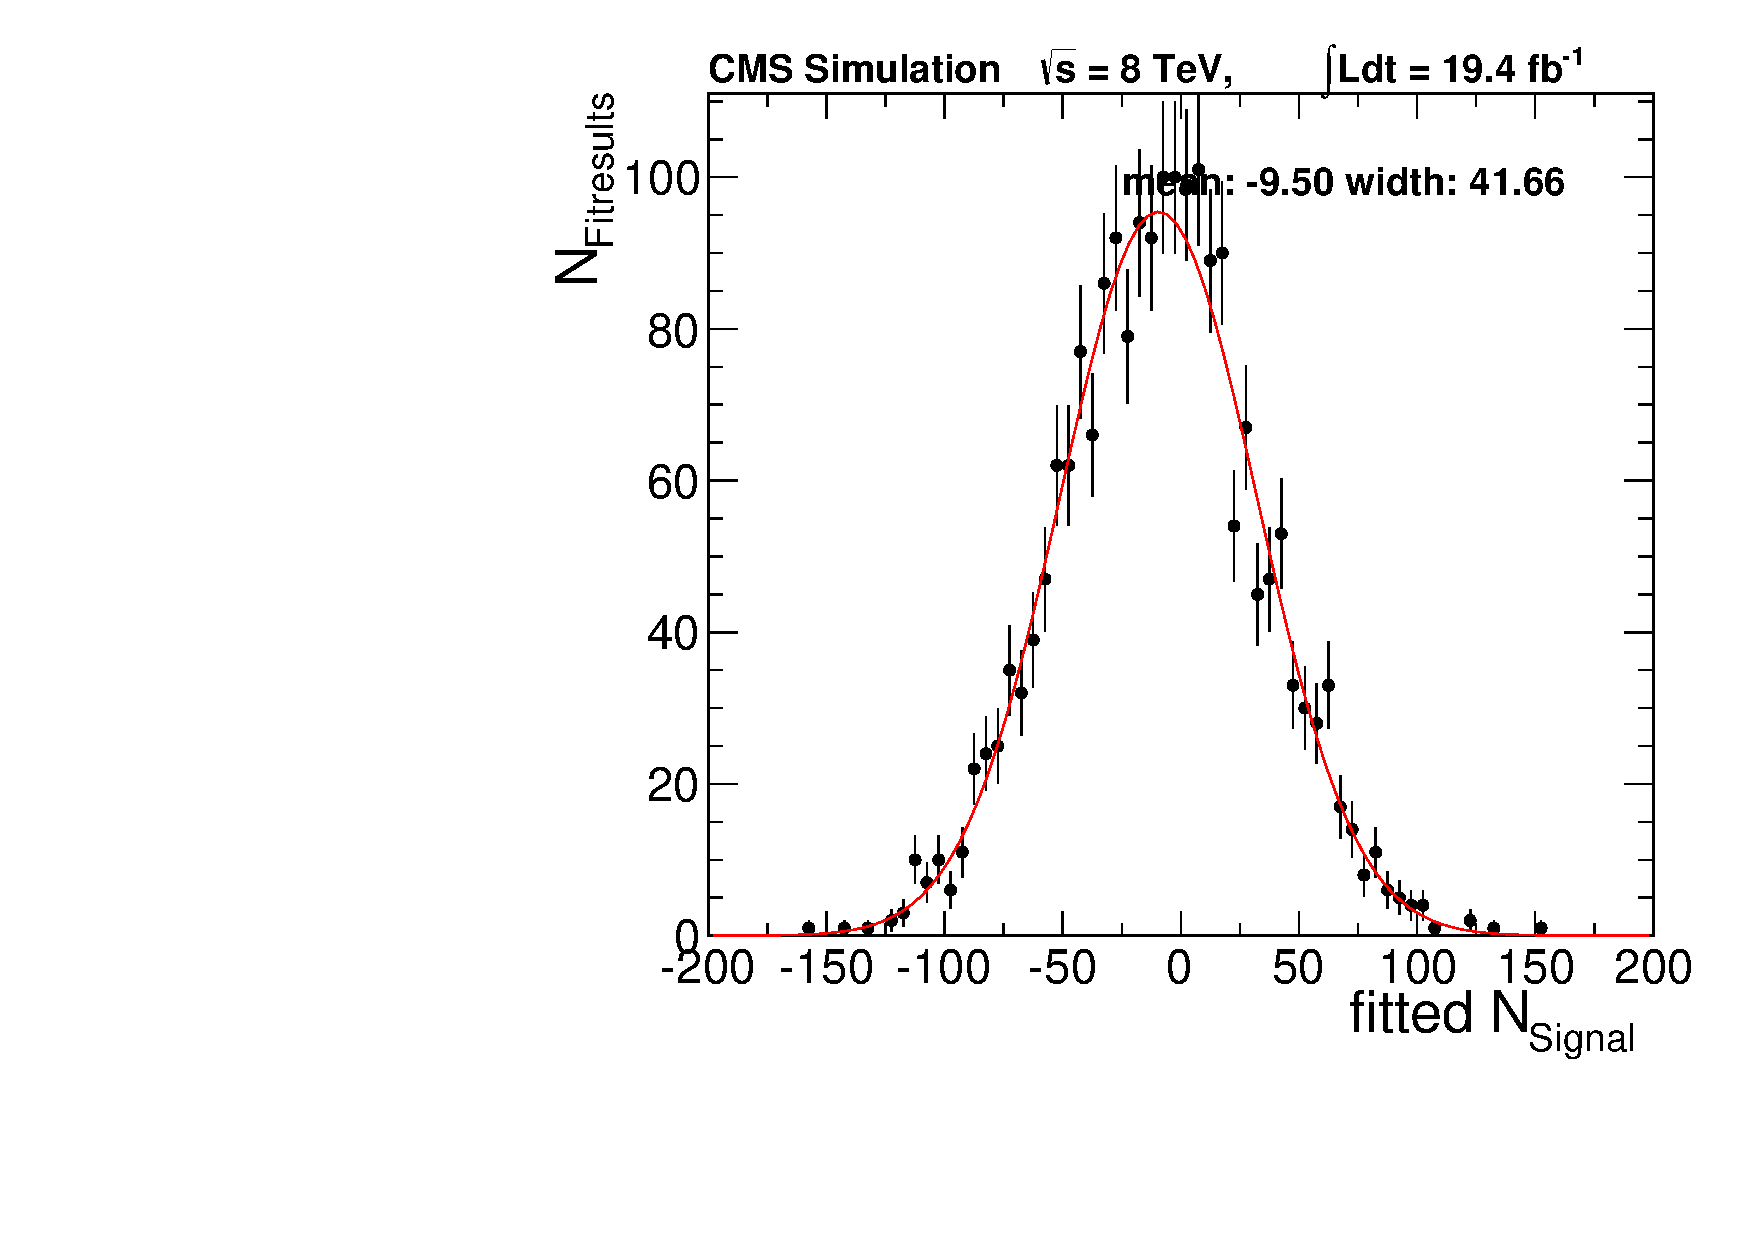
\includegraphics[width=\textwidth]{plots/results/fit/nSPure_backgroundOnly_Fixedm078.pdf}
  \end{minipage}
  \begin{minipage}[t]{0.49\textwidth}
    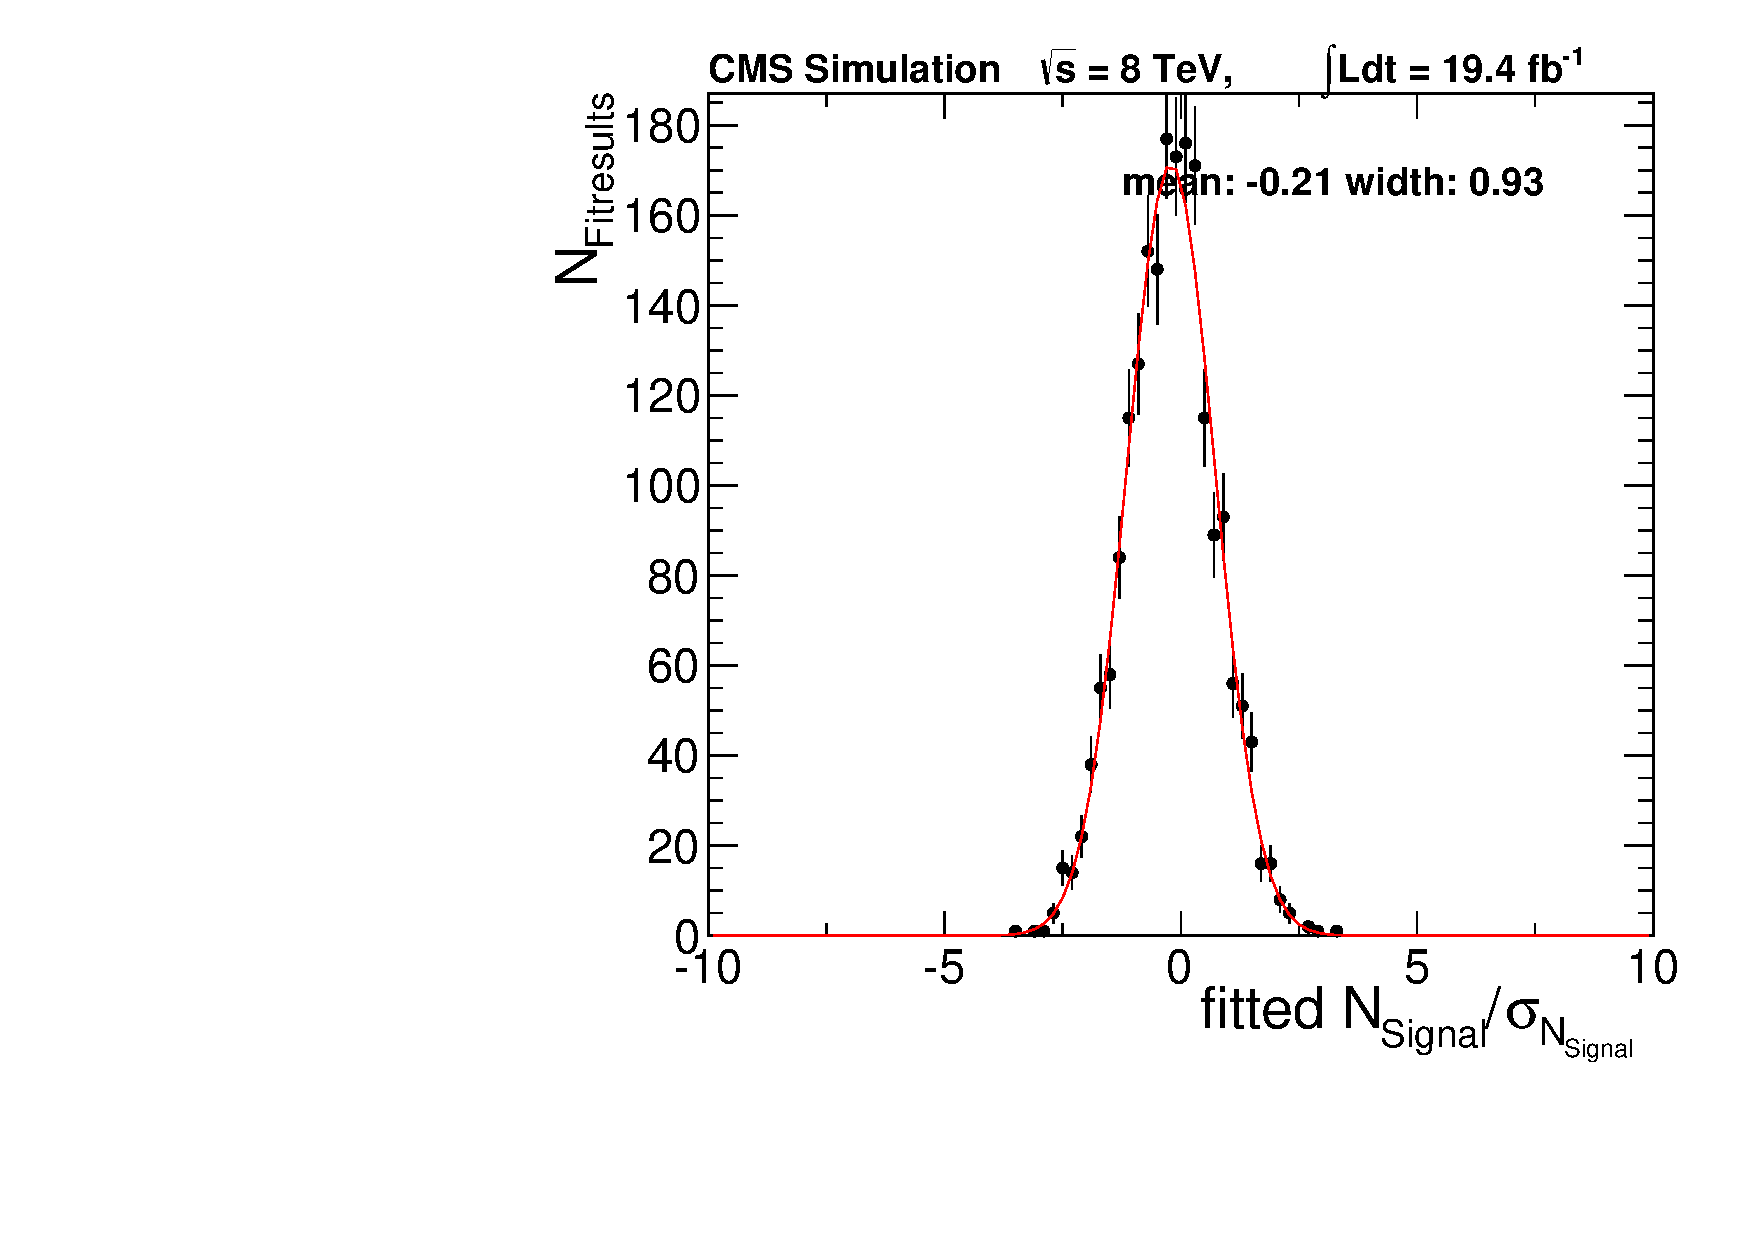
\includegraphics[width=\textwidth]{plots/results/fit/nS_backgroundOnly_Fixedm078.pdf}
  \end{minipage}

  \caption{Distribution of fit observables in toy studies for background only toys with fixed edge position. Shown are the fitted number of signal events in the central region (left) and the fitted number of signal events divided by the fitted uncertainty in the central region (right).}
  \label{fig:toys:backgroundOnlyFixed}
\end{figure}
\paragraph{Toy studies with signal injection}
The fit performance in the presence of a signal is tested by injection a signal of 120 events with and edge position of 78 GeV, both in the central and in the forward signal region. Figure \ref{fig:toys:signalInjected} show the resulting distribution of fit results for a selection of observables in the central signal region. The distribution of the number of signal events can be fit with a Gaussian with a mean of 114.42 events and a width of 44.13 events. Divided by the fitted uncertainty this gives a Gaussian with mean of 2.5 and a with of about 1. The edge position is fitted to be 78 GeV with a width of 2 GeV. We conclude that the fit performs well in the presence of a signal and is able to reproduce the injected signal parameters on average. 

\begin{figure}[hbp]
  \centering
  \begin{minipage}[t]{0.49\textwidth}
    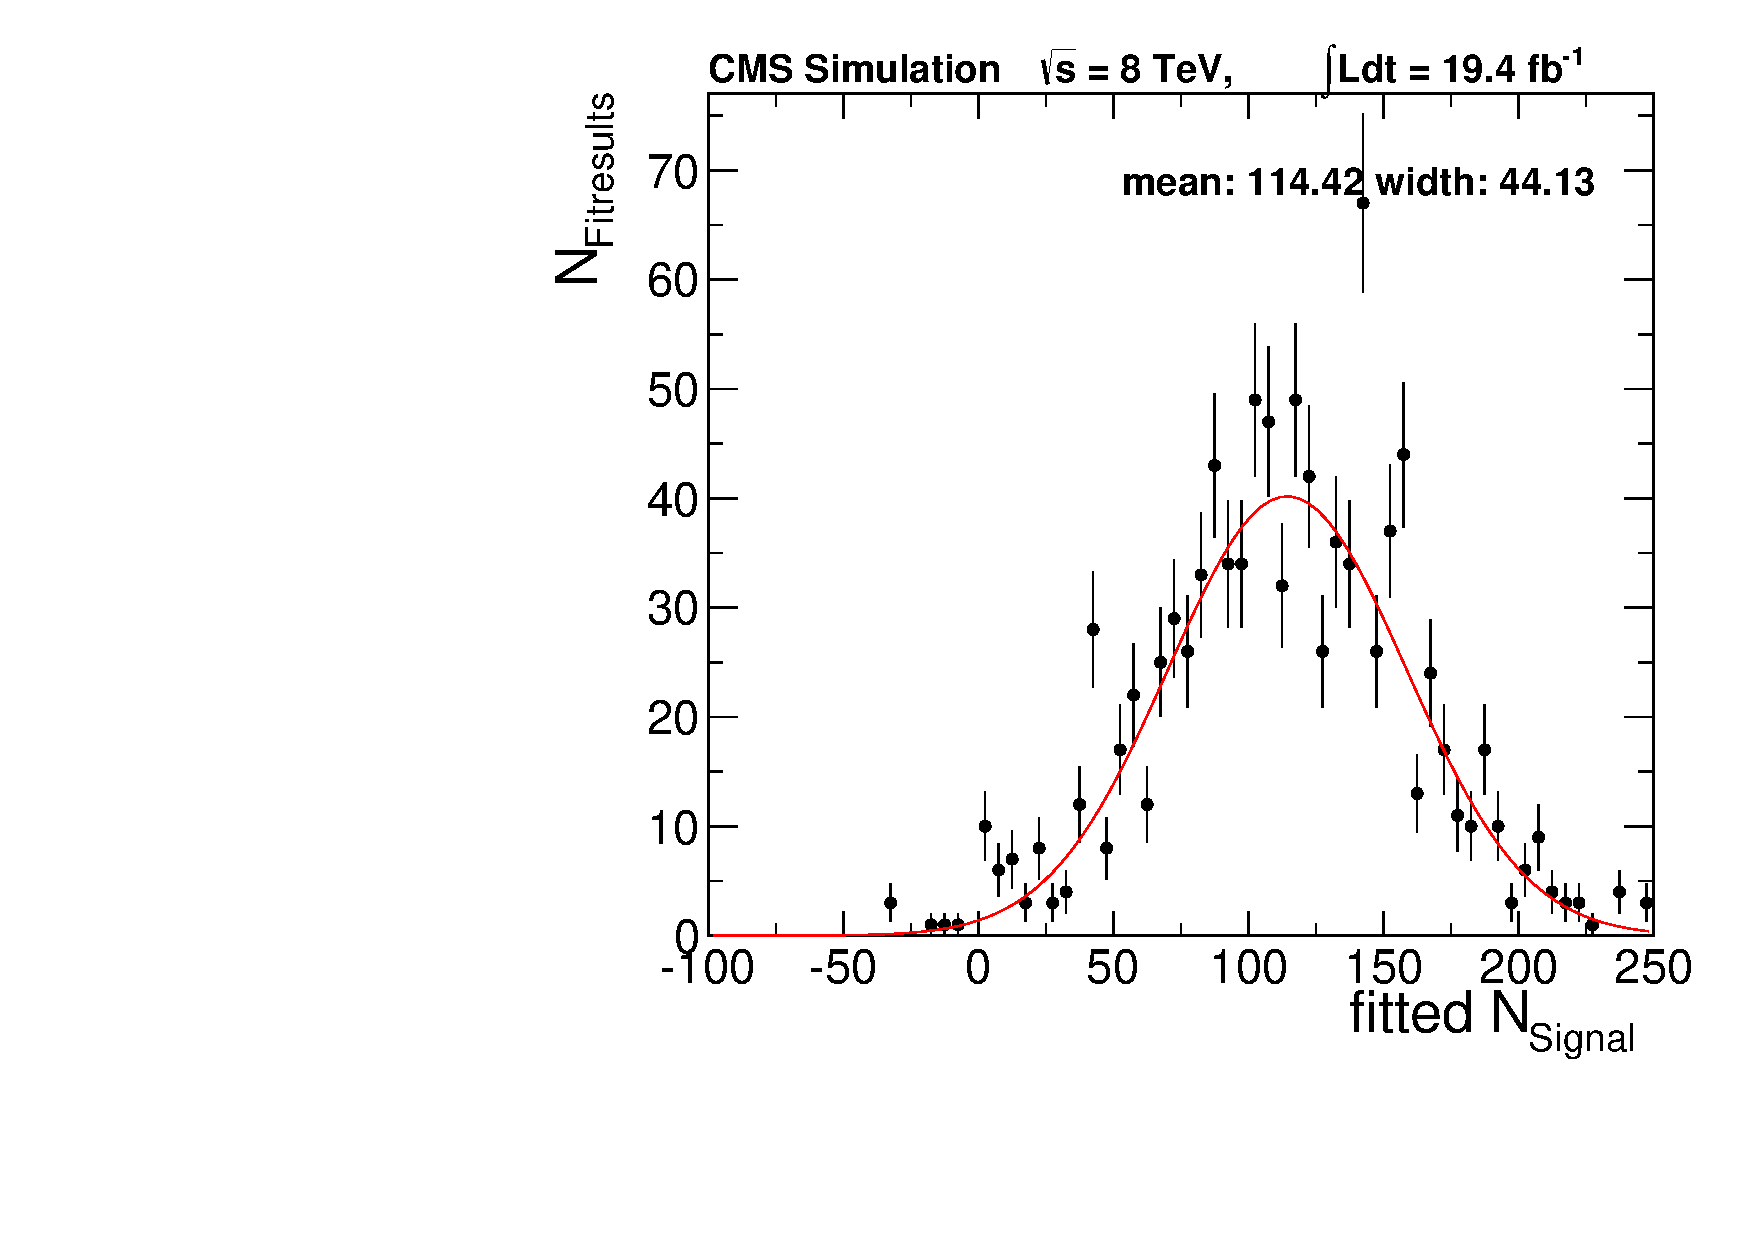
\includegraphics[width=\textwidth]{plots/results/fit/nSPure_signal120_m078.pdf}
  \end{minipage}
  \begin{minipage}[t]{0.49\textwidth}
    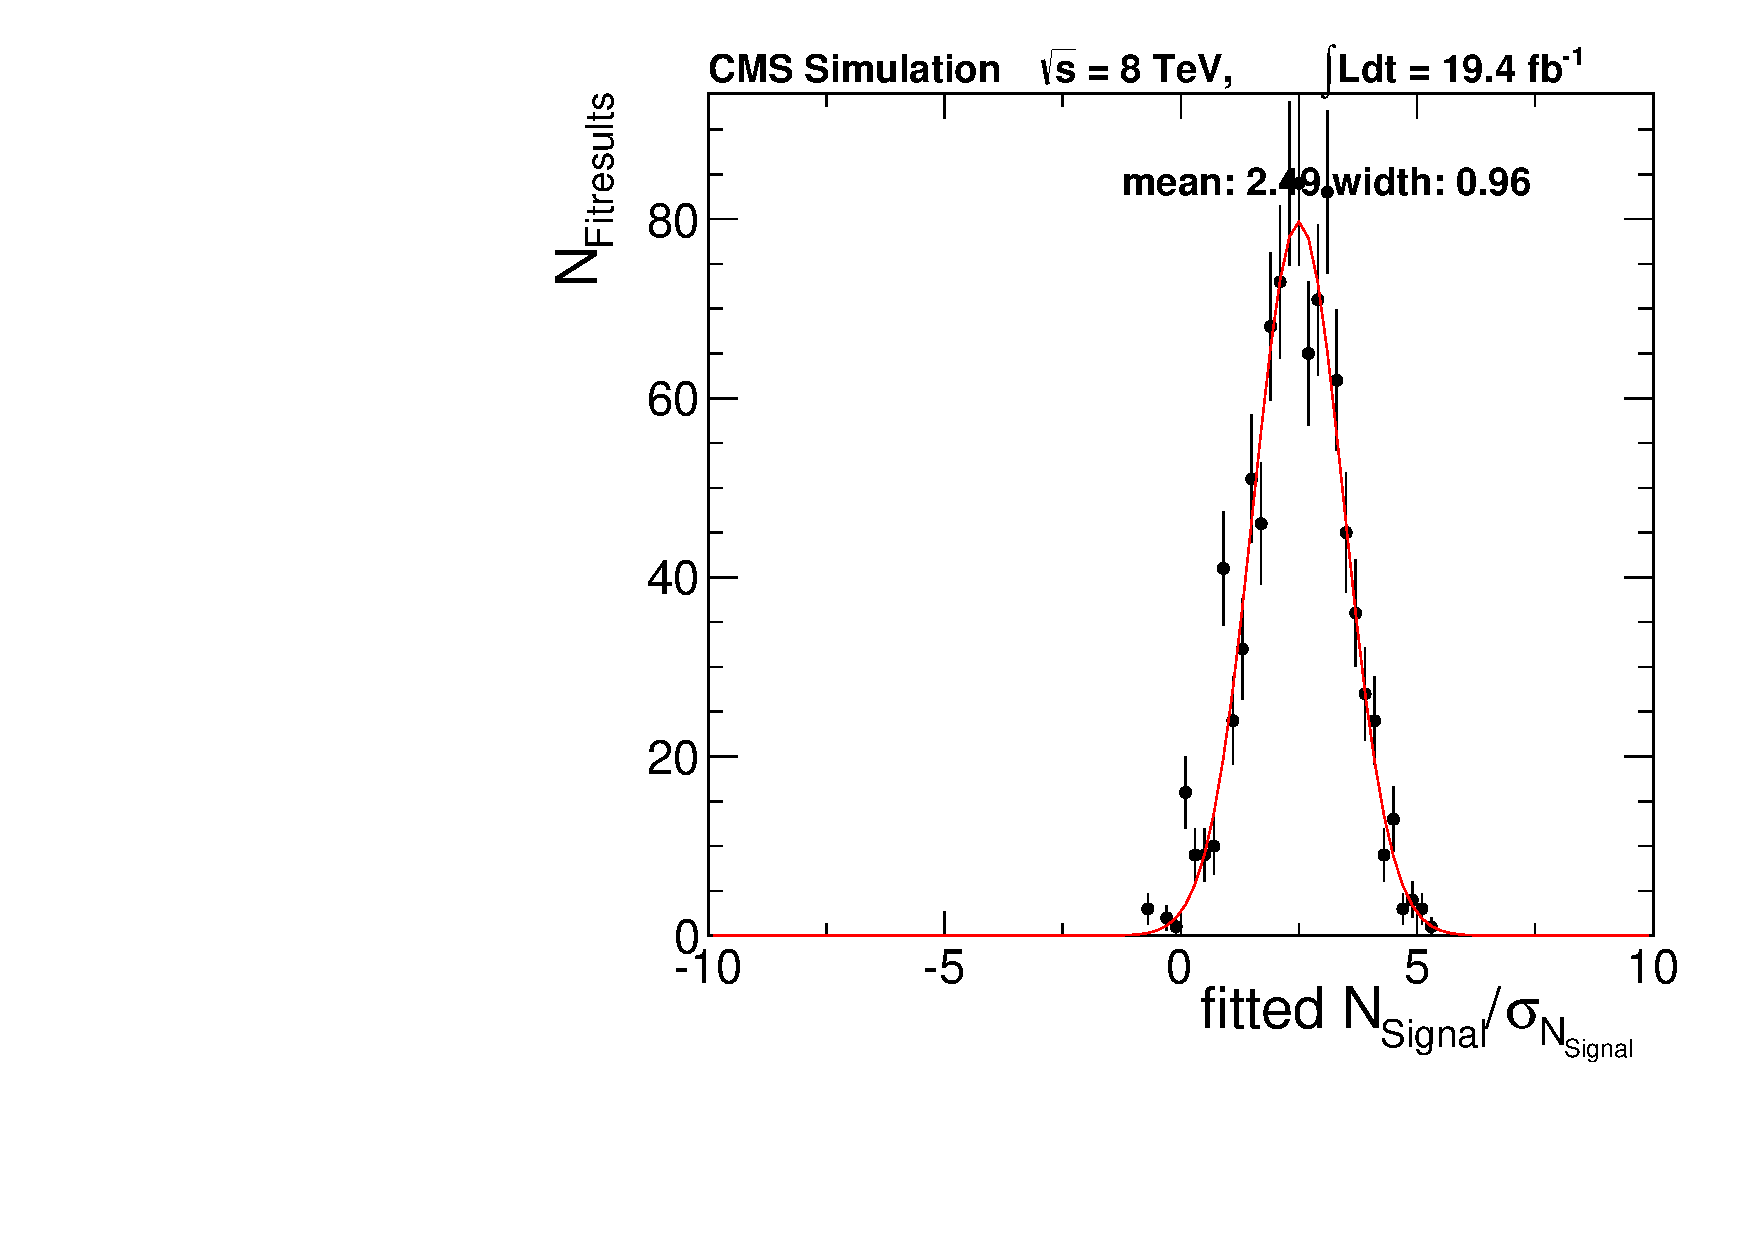
\includegraphics[width=\textwidth]{plots/results/fit/nS_signal120_m078.pdf}
  \end{minipage}
  \begin{minipage}[t]{0.49\textwidth}
    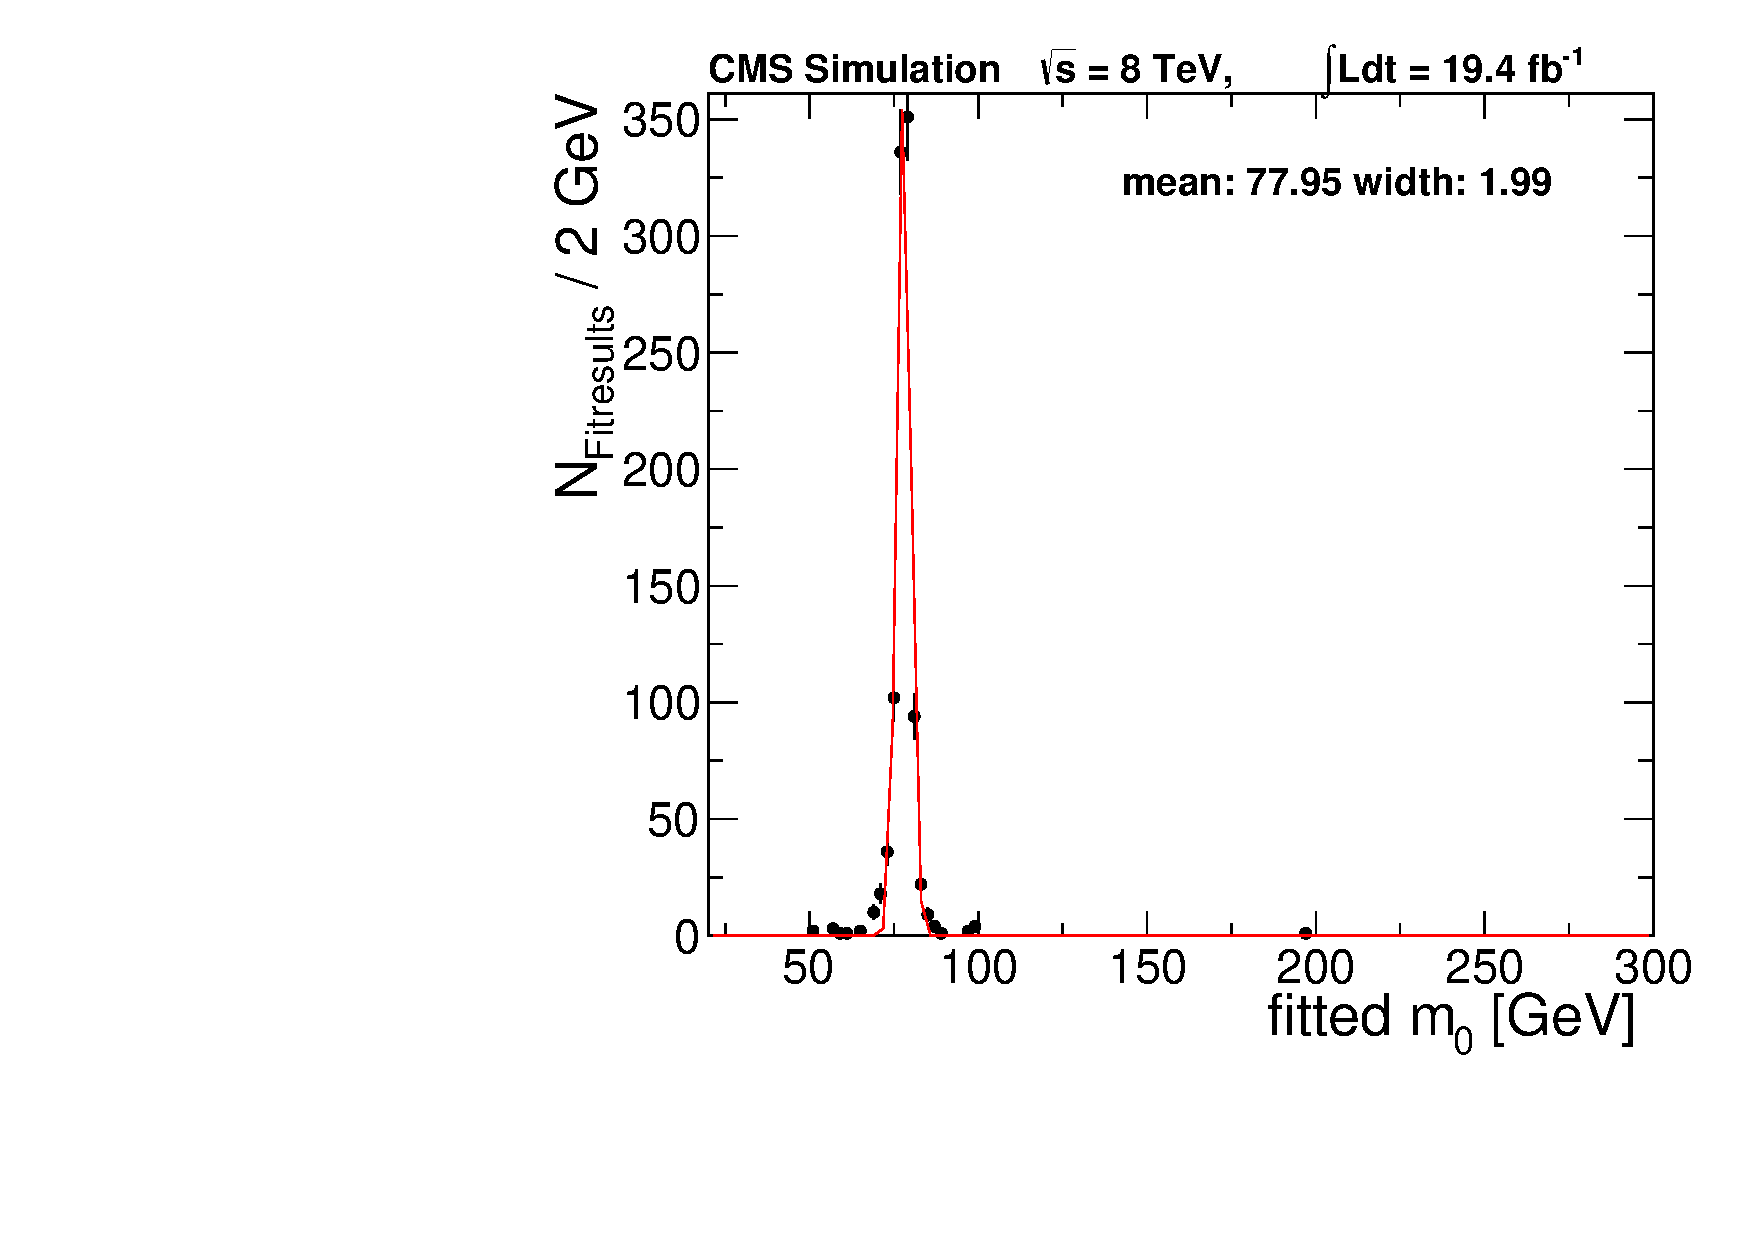
\includegraphics[width=\textwidth]{plots/results/fit/m0_signal120_m078.pdf}
  \end{minipage}
  \begin{minipage}[t]{0.49\textwidth}
    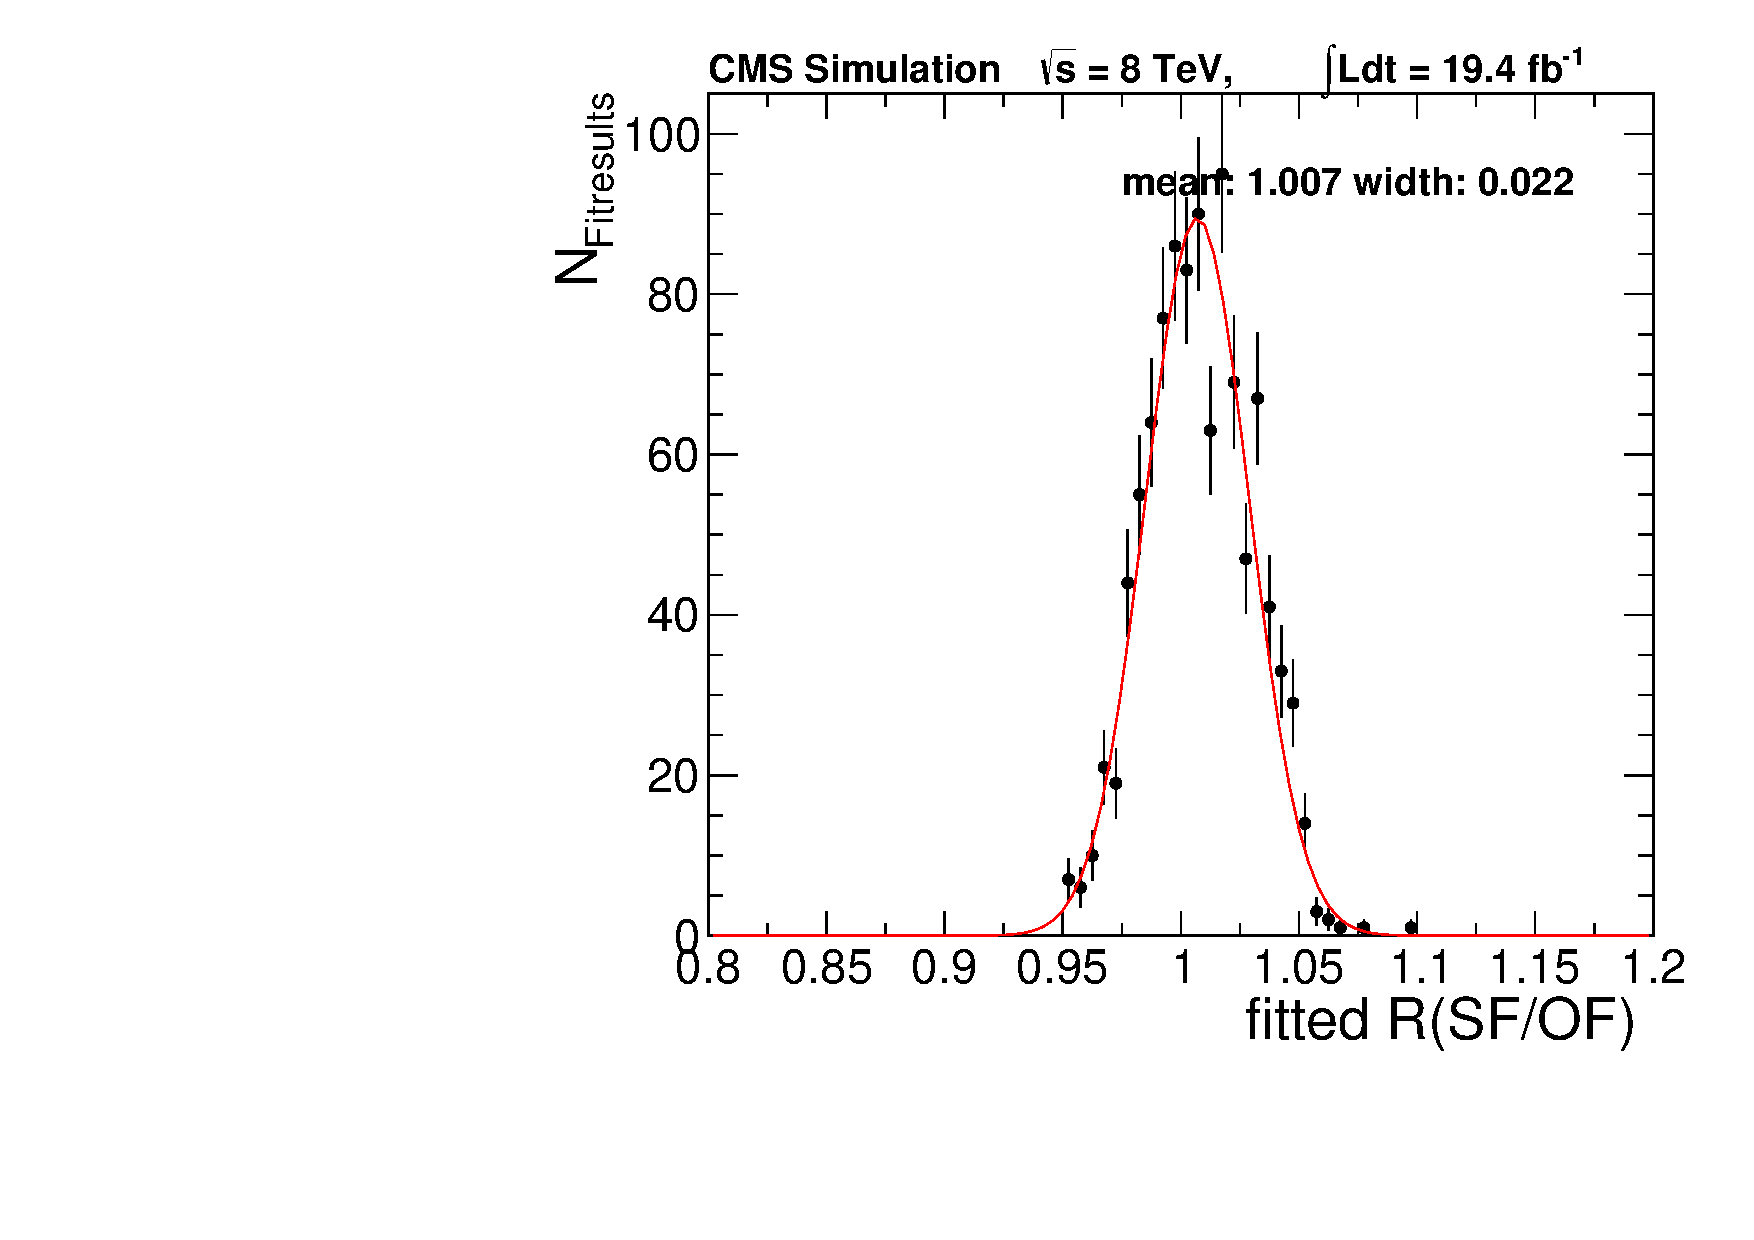
\includegraphics[width=\textwidth]{plots/results/fit/rSFOF_signal120_m078.pdf}
  \end{minipage}
  \caption{Distribution of fit observables in toy studies with a signal injected. Shown are the fitted number of signal events in the central region (upper left), the fitted number of signal events divided by the fitted uncertainty in the central region (upper right), the fitted edge position (lower left) and the fitted \Rsfof in the central region (lower right).}
  \label{fig:toys:signalInjected}
\end{figure}